
\section{Advanced Cryptography}

\subsection{Data at rest}

\subsubsection{Searchable Encryption}

\paragraph{Searchable Encryption}
consists of three protocols:
\begin{enumerate}
\item Setup:
Client generates an \emph{encrypted database + encrypted search index}%
\footnote{A search index is a mapping from document ids to keywords, and/or vice versa.
For more details see the lecture \textit{Information Retrieval}.},
uploads them to the server.
\item Search:
Client generates a \emph{search token}, server uses it to process the search, returns the result.
\item Update:
Client generates an \emph{update token}, server uses it to update the encrypted database and encrypted search index, returns success/failure.
\end{enumerate}
%
Active field of research, many open problems (e.g. leakage analysis + prevention).

\paragraph{Goals}
\begin{itemize}
\item Security:
Confidentiality (of data and queries) against an \emph{honest-but-curious} server.%
\footnote{Compare this security model against a fully malicious server.}
\item Efficiency:
Storage, computational, bandwidth requirements.
\item Functionality:
Supported query types.
\end{itemize}

\paragraph{First construction}
Idea: randomly choose a PRF $F_K$ and replace each keyword $w$ in the index by $F_K(w)$.
Also encrypt each document under some symmetric key $K_0$.

Leakage from setup $\mathcal{L}_{Setup}$:
total number of documents and keywords, keyword frequency, co-occurences of keywords.

Leakage from searches $\mathcal{L}_{Search}$:
result patterns, query patterns, result intersection between queries.

\begin{figure}[h]
    \centering
	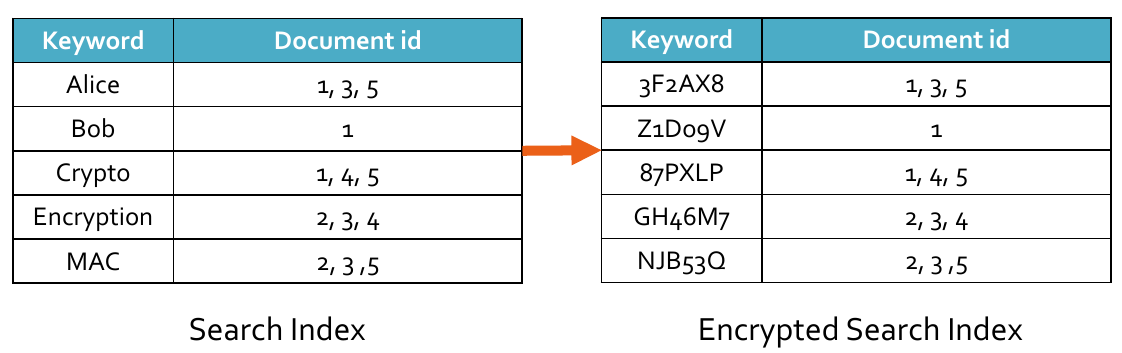
\includegraphics[scale=0.4]{images/searchable-encryption-1.png}
    \caption{First construction for searchable encryption}
    \label{fig:searchable-encryption-1}
\end{figure}

\paragraph{Second construction}
Idea: randomly choose a PRF $F_K$.
For each keyword $w$ calculate $K_1 || K_2 = F_K(w)$.
Replace each keyword with $K_1$ (as before).
In addition: associate each document id for $w$ with a counter $cnt$ and replace the id with $id \xor F_{K_2}(cnt)$.

This hides the co-occurences of keyword pairs (PRF security).

\begin{figure}[h]
    \centering
	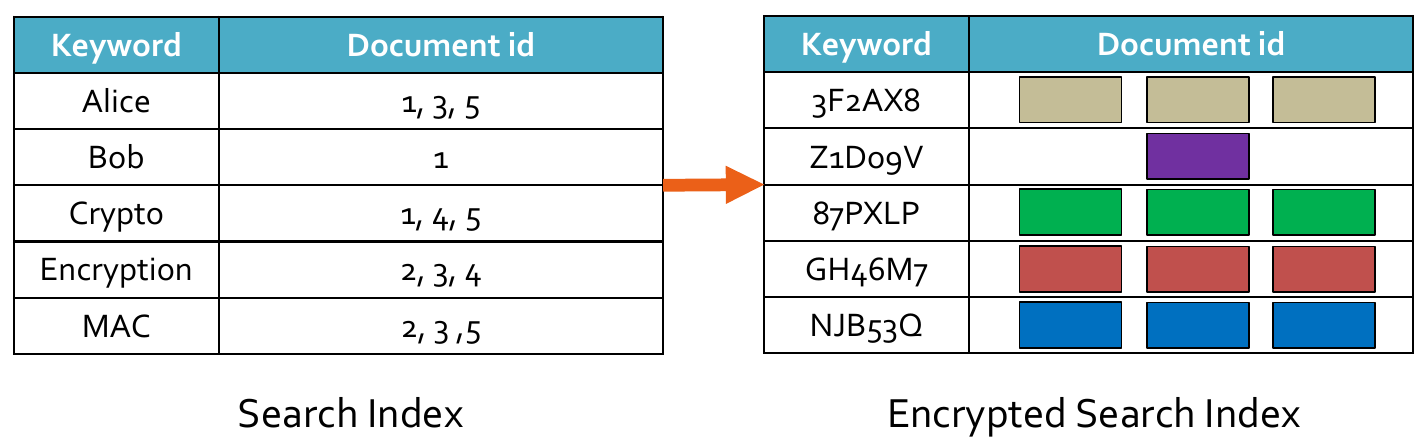
\includegraphics[scale=0.35]{images/searchable-encryption-2.png}
    \caption{Second construction for searchable encryption}
    \label{fig:searchable-encryption-2}
\end{figure}

\paragraph{Third construction}
Idea: ... (as before) ... \\
In addition: associate each document id for $w$ with a counter $cnt$ and replace the id with $id \xor F_{K_2}(cnt)$.
Then store this document id value in a key-value store (dictionary) under ``key'' $F_{K_1}(cnt)$.

Search:
Send $(K_1, K_2, |cnt_{querystring}|)$ to the server.
Server recomputes the $F_{K_1}(cnt)$ to find the values in the dictionary.
Then decrypts them to document ids using $K_2$.
Looks up the encrypted documents and returns them.

Leakage from setup $\mathcal{L}_{Setup}$:%
\footnote{This is also what an adversary learns from a single snapshot.}
total number of documents.

Leakage from searches $\mathcal{L}_{Search}$:
(same as before) result patterns, query patterns, result intersection between queries.

\begin{figure}[h]
    \centering
	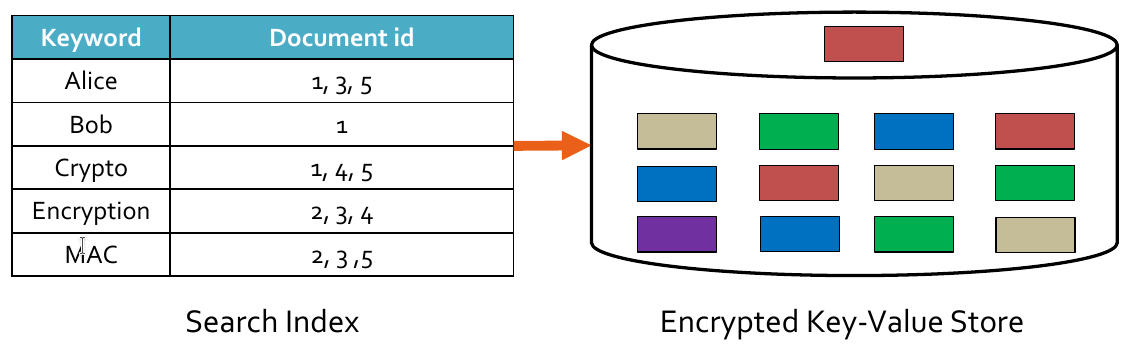
\includegraphics[scale=0.4]{images/searchable-encryption-3.png}
    \caption{Third construction for searchable encryption (setup)}
    \label{fig:searchable-encryption-3}
\end{figure}
\begin{figure}[h]
    \centering
	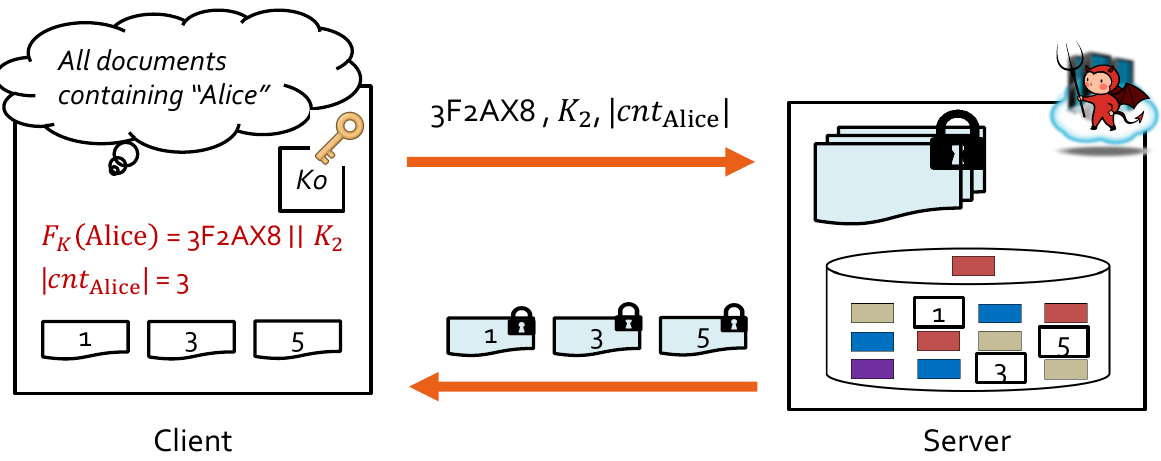
\includegraphics[scale=0.4]{images/searchable-encryption-4.png}
    \caption{Third construction for searchable encryption (search)}
    \label{fig:searchable-encryption-4}
\end{figure}

\paragraph{Defining Leakage}
Goal: formally define the leakage $\mathcal{L} = (\mathcal{L}_{Setup}, \mathcal{L}_{Search})$ of searchable encryption schemes.

Security game: an adversary $\A$ interacts with a challenger $\C$ that contains either the real world or a simulator.
The simulator $\mathcal{S}$ only has access to the leakage $\mathcal{L}$ (but not to the secret key).
Intuitively, the adversary should gain no extra information other than the leakage.

\begin{figure}[h]
    \centering
	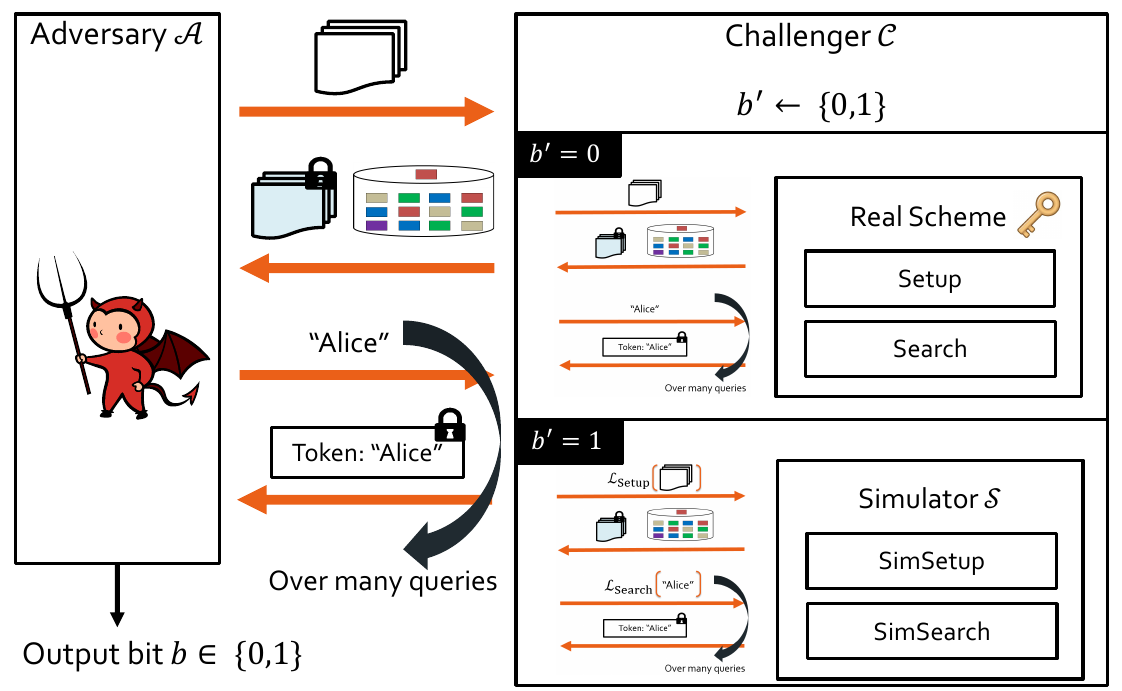
\includegraphics[scale=0.4]{images/searchable-encryption-leakage.png}
    \caption{Searchable encryption leakage game}
    \label{fig:searchable-encryption-leakage}
\end{figure}

\paragraph{Analysing Leakage}
What can the adversary infer from the leakage?
It turns out that given auxiliary information, one can e.g. perform query recovery.


\subsection{Data in transit}

\subsubsection{Transport Layer Security TLS}

\paragraph{Goal} ``Secure channel between two peers'' --
confidentiality, authentication, integrity in the face of a network adversary
and only requiring a reliable in-order transport mechanism.

\paragraph{Architecture}
\begin{itemize}
\item Handshake protocol:
Cipher suite negotiation, peer authentication, key material establishment
\item Record protocol:
``normal'' data transfer
\item Many other features: session resumption, renegotiation, extensions, ...
\end{itemize}

For the format of the handshake protocol and a TLS record,
see \autoref{fig:tls-handshake} and \autoref{fig:tls-record}.
These blueprints are instantiated using the negotiated cipher suite:
for example RSA for the key exchange and authentication with AES128-CBC as a cipher and SHA1 as a MAC.

\emph{Ad handshake}:
the peers create/derive a pre-master secret during the handshake.
Authentication is done via a signature over the entire handshake transcript (\texttt{ServerCertificateVerify}).
MITM protection via MAC over transcript (\texttt{ServerFinished}).
This is an example of \emph{Sign-and-Mac}.

\begin{figure}[h]
    \centering
	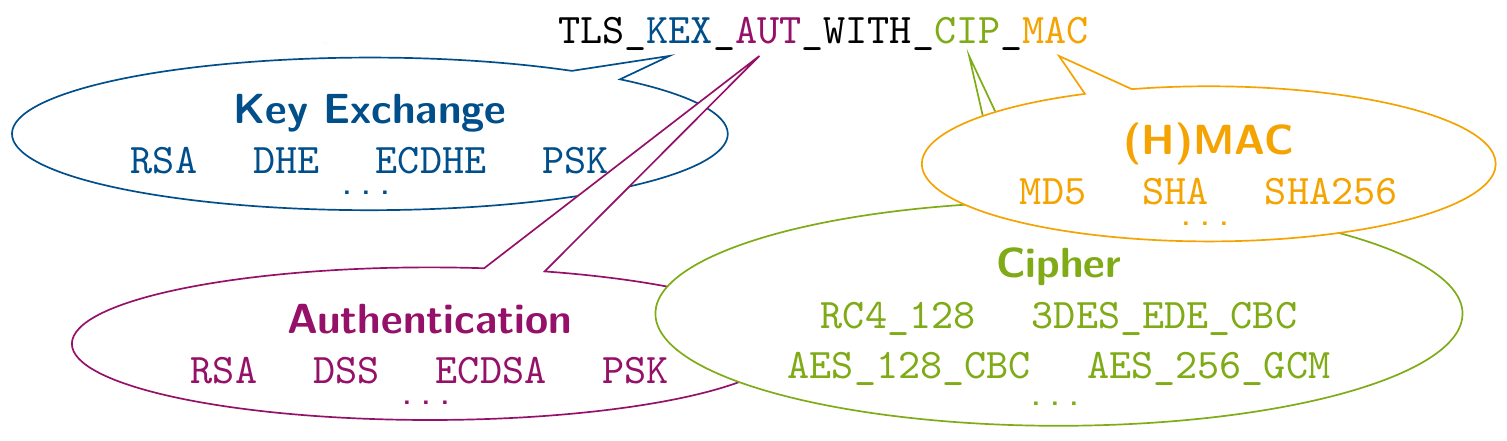
\includegraphics[scale=0.3]{images/tls-cipher-suite.png}
    \caption{TLS Cipher Suite Format ($\leq$ TLS 1.2)}
    \label{fig:tls-cipher-suite}
\end{figure}

\begin{figure}[h]
    \centering
	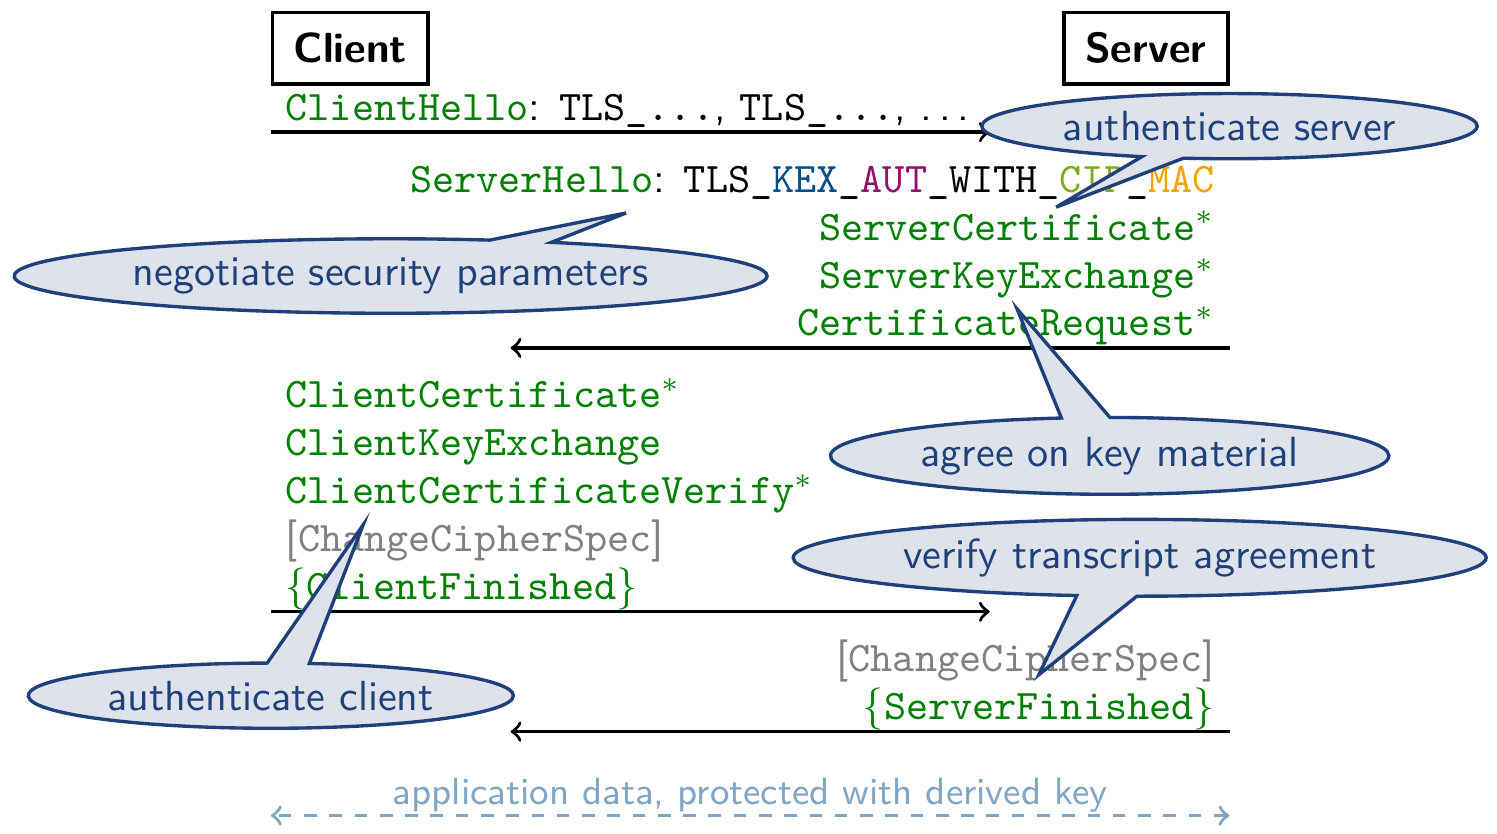
\includegraphics[width=0.6\textwidth]{images/tls-handshake-12.png}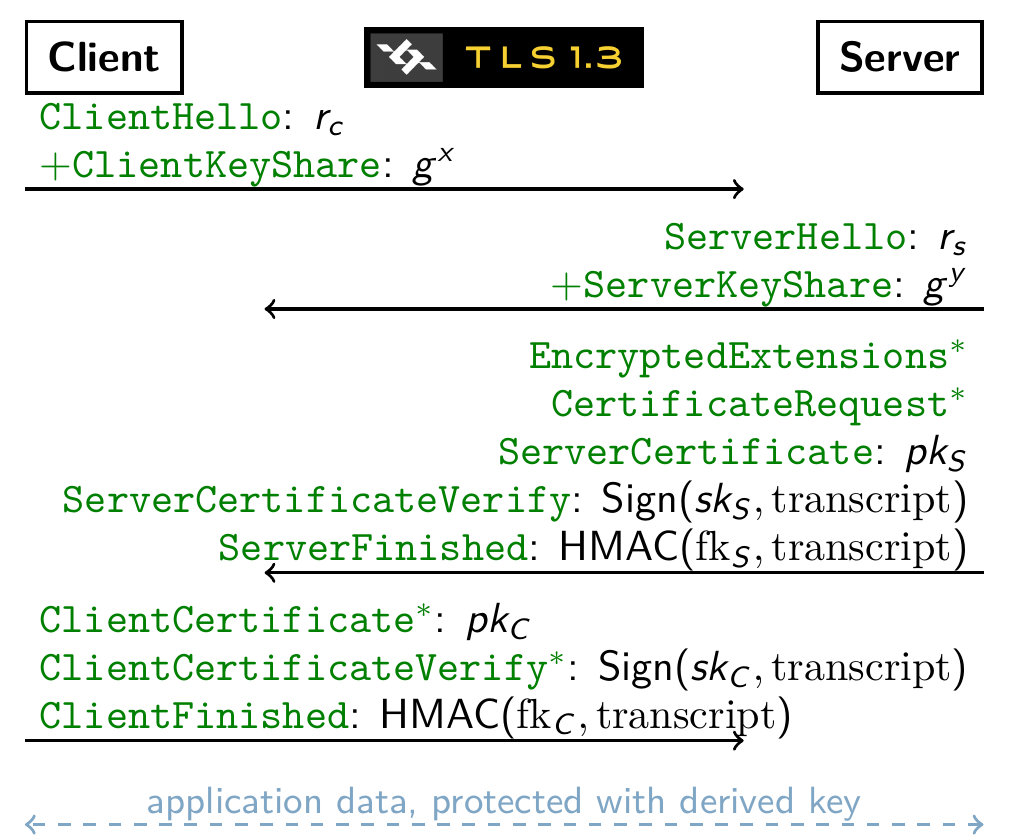
\includegraphics[width=0.4\textwidth]{images/tls-handshake-13.png}
    \caption{TLS Handshake Protocol (simplified, left: $\leq$ TLS 1.2 right: TLS 1.3)}
    \label{fig:tls-handshake}
\end{figure}

\begin{figure}[h]
    \centering
	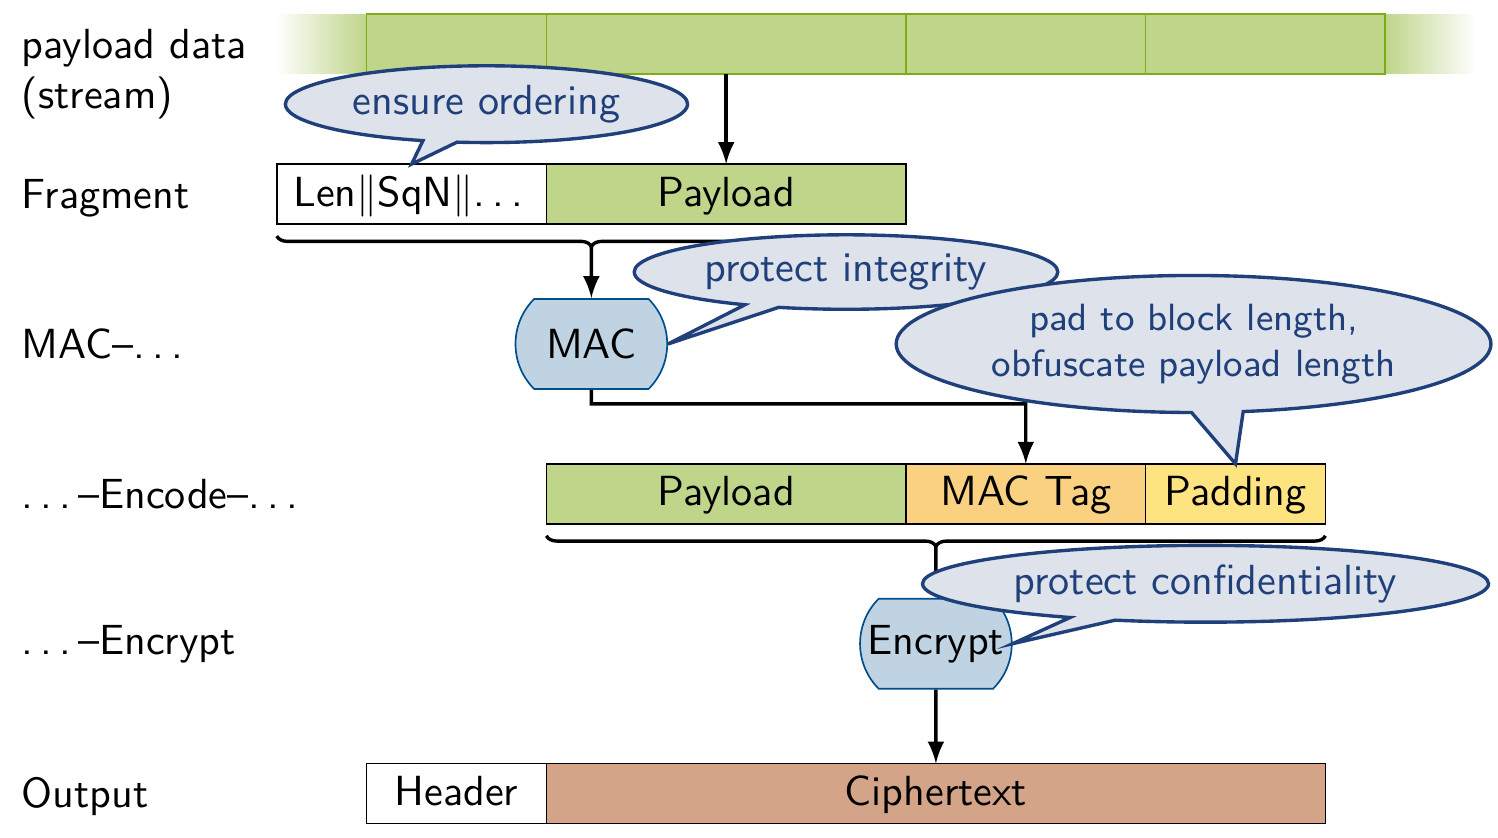
\includegraphics[width=0.5\textwidth]{images/tls-record-12.png}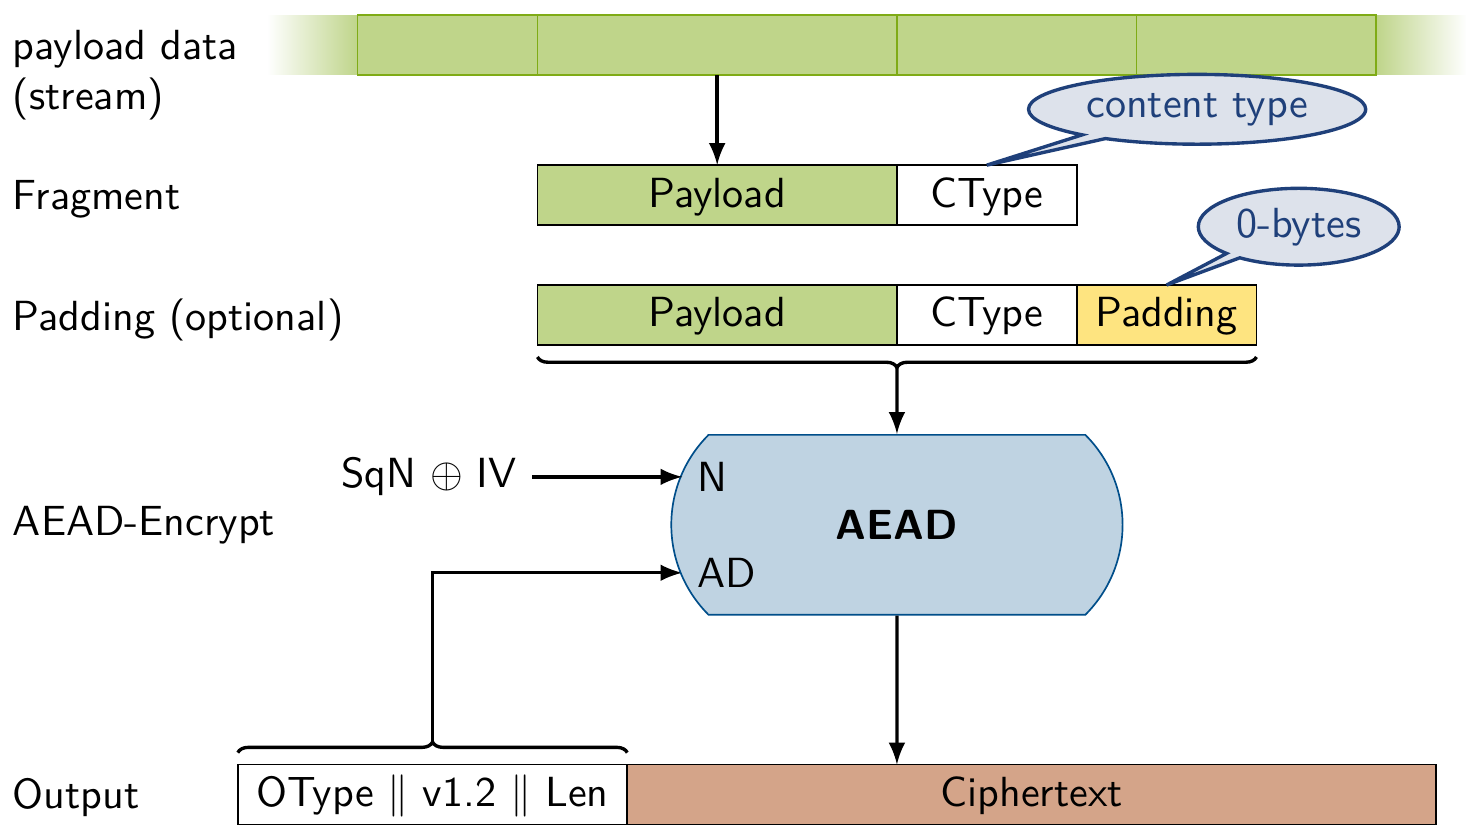
\includegraphics[width=0.5\textwidth]{images/tls-record-13.png}
    \caption{TLS Record Format (simplified, left: $\leq$ TLS 1.2 right: TLS 1.3)}
    \label{fig:tls-record}
\end{figure}

\paragraph{Security Issues}
Various, due to protocol complexity.
Protocol issues, padding oracles, implementation bugs, downgrade attacks.

\paragraph{TLS 1.3 Goals}
\begin{itemize}
\item \emph{Clean up:}
remove legacy crypto, unused/broken features, static RSA/DH\footnote{They don't provide forward secrecy.}
\item \emph{Improved latency:}
TLS 1.2 handshake takes 2 round trips, ``wasting'' one to learn server capabilities.
Instead, run full hand-shake in 1 round trip (possible due to feature reduction).
0-RTT handshake using a shared resumption secret PSK
-- at the sacrifice of FS and danger of replay attack.
\item \emph{Improved privacy:}
Encrypt all most all handshake messages.
Send a \texttt{[Client|Server]KeyShare} with the \texttt{[Client|Server]Hello}.
Then encrypt all subsequent messages with the \emph{handshake traffic key} $tk_{hs}$.
\item \emph{Continuity:}
Interoperability (make \texttt{ClientHello} look like in TLS 1.2)
\item \emph{Security assurance:}
Formally analyse the protocol before it is deployed (rather than after).
This is done in various ways: computational model, tool-based, verified implementations.
\end{itemize}

\paragraph{Key Separation}
Detailed key schedule for deriving separate keys everywhere.
Advantage: if a \emph{key} is compromised, all other keys still remain secure
(as long as the \emph{secrets} from which they were derived are private).
\\
In TLS 1.3: use $HKDF.Extract(salt, keymaterial)$ to extract entropy (e.g. from PSK)
into a random key which can be expanded into longer random output using $HKDF.Expand(key, context, length)$.
\\
E.g. master secret MS, resumption master secret RMS, exporter master secret EMS,
application data traffic key $tk_{app}$, ...


\subsubsection{Signal Messaging Protocol}

TODO


\subsubsection{Messaging Layer Security Protocol}

TODO


\subsection{Data under computation}

\subsubsection{Fully Homomorphic Encryption FHE}

\paragraph{Motivation}
Allow data to be processed while remaining encrypted.
Applications: Secure Outsourcing, Private Set Intersection (PSI), Private Machine Learning As A Service.

\paragraph{Challenges}
\begin{itemize}
\item Crypto: Underlying math, parameter selection, security analysis.
\item Computation Paradigm: No if/else, no loops, no jumps -- all would leak
information about the encrypted data. Optimisations, approximations, SIMD batching.
\end{itemize}

\paragraph{(Ring-) Learning With Errors (R)LWE}
The LWE problem is conjectured to be hard (even on quantum computers).
Simplified idea: mask data with random noise.
Need to carefully define encryption/decryption, addition and multiplication.
For multiplication, we need \emph{relinearization} to make the maths work.

Problem: noise increases with each operation and will eventually grow too large for decryption to succeed.
Solution: use \emph{bootstrapping} to (homomorphically) reduce the noise again.
Effectively, bootstrapping produces an encryption of the same encrypted message,
but at a lower noise level.\footnote{This is one of the practical breakthroughs of Gentry '09.}
But: bootstrapping is complex and slow (order of seconds to minutes), so we try to avoid it in practice.

\begin{figure}[h]
    \centering
	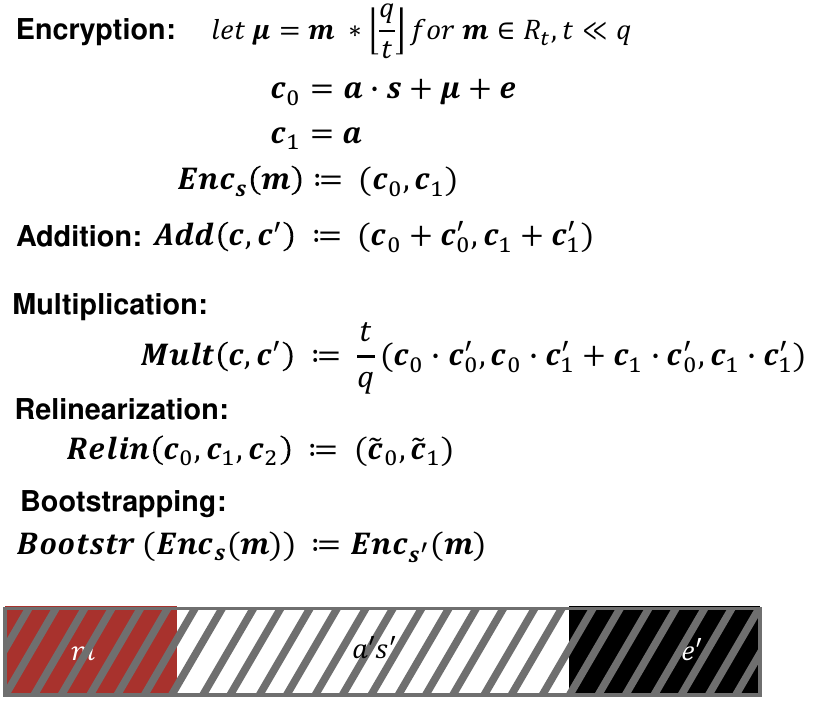
\includegraphics[scale=0.4]{images/fhe-rlwe.png}
    \caption{FHE: RLWE operations}
    \label{fig:fhe-rlwe}
\end{figure}

\paragraph{Parameter selection}
Careful trade-off between efficiency, security and correctness.
Security based on current knowledge on how hard the LWE problem is.

\paragraph{Tool support}
``Libraries'' implement the underlying FHE schemes, addressing the crypto side.
``Compilers'' help with writing higher-level code, addressing the computation paradigm concerns.
E.g. SEAL (C++), EVA (Python), nGraph-HE (Tensorflow), SEALion (Keras).

